\sectionframe{Modeling}

\begin{frame}
 \frametitle{Example: production problem (Lewig Sanstetten)}
 \begin{figure}
  \centering
  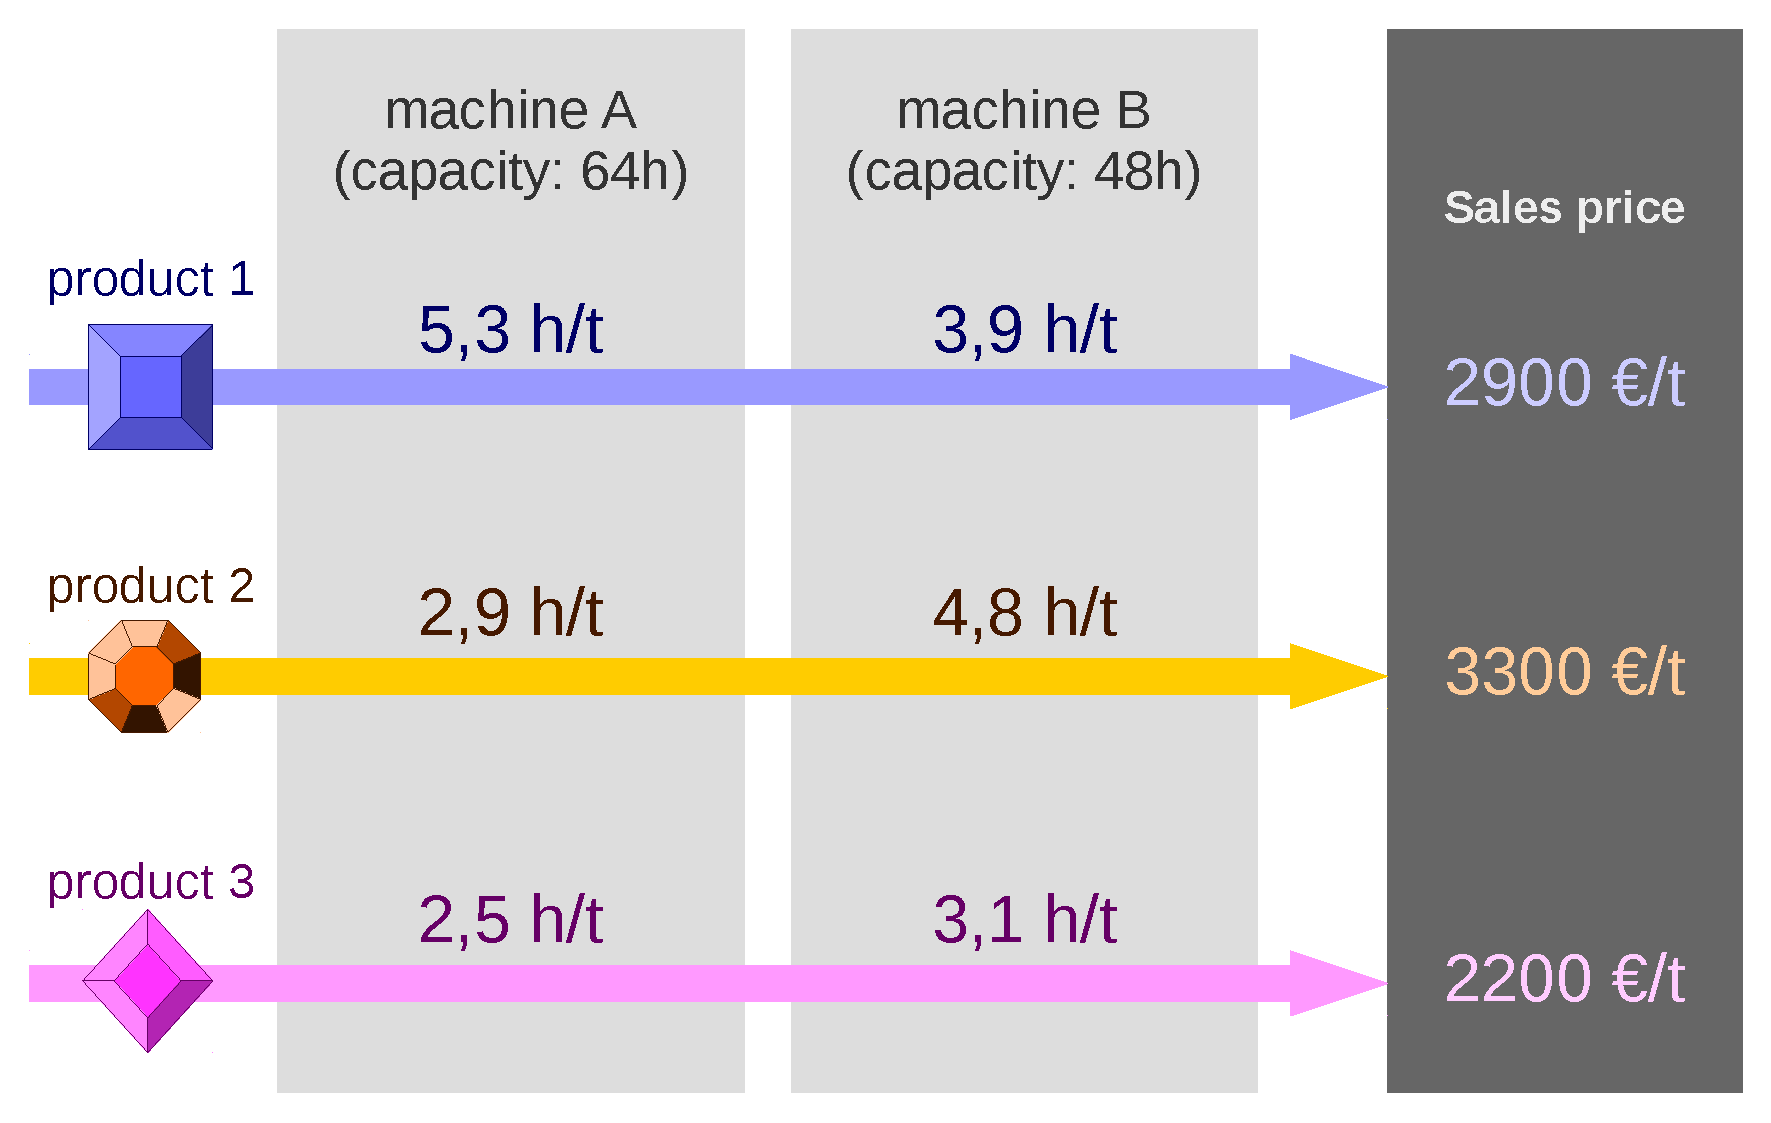
\includegraphics[width=\linewidth]{Bilder/LewigSanstetten}
 \end{figure}
 
 How much of each product should be produced?
\end{frame}

\begin{frame}
 \frametitle{What is a model?}
 \begin{itemize}
  \item abstract description of a real system
  \item for exmaple useful for
  \begin{itemize}
   \item system design
   \item performance analysis
   \item \textbf{decision support}
  \end{itemize}
  \item guideline: as exact as necessary, as simple as possible
 \end{itemize}
\end{frame}

\begin{frame}
 \frametitle{Mathematical optimization models for decision support}
 Components of a mathematical optimization model\footnote{also: mathematical program\\}:
 \begin{description}\footnotesize
  \item[decision variables] system items which can be set by the decision maker 
  \begin{itemize}
   \item in the example: the production quantities of the products
  \end{itemize}
  \item[constraints] restrictions which have to be satisfied by the decision variables to get a proper solution
  \begin{itemize}
   \item in the example: the capacity of the machines may not be exceeded
  \end{itemize}  
  \item[objective function] a function of the decision variables, which the decision maker has to optimize, i.e. minimize or maximise
  \begin{itemize}
   \item in the example: the total revenue
  \end{itemize}  
 \end{description}
\end{frame}

\begin{frame}
 \frametitle{Example: production problem -- decision variables}
 \begin{description}
  \item[$x_1$] production quantity of product~1
  \item[$x_2$] production quantity of product~2
  \item[$x_3$] production quantity of product~3
 \end{description}
 
 \begin{block}{Definition: Solution of an optimization model}
  By assigning specific values to the decision variables, we get a solution for the model.
 \end{block}
\end{frame}

\begin{frame}
 \frametitle{Example: production problem -- constraints}
  
  Capacity of machine~A may not be exceeded:
  \begin{itemize}
   \item $5,3 \cdot x_1 + 2,9 \cdot x_2 + 2,5 \cdot x_3 \leq 64$
  \end{itemize}

  Capacity of machine~B may not be exceeded:
  \begin{itemize}
   \item $3,9 \cdot x_1 + 4,8 \cdot x_2 + 3,1 \cdot x_3 \leq 48$
  \end{itemize}
 
 \begin{block}{Definition: Feasible Solution of an optimization model}
  A solution which satisfies all constraints is called a feasible solution. The set of all feasible solution is called solution space. 
 \end{block}
\end{frame}

\begin{frame}
 \frametitle{Example: production problem -- objective function}
 Maximize the revenue (in k€):
 \begin{itemize}
  \item $\max U(x_1, x_2, x_3) = 2,9\cdot x_1 + 3,3\cdot x_2 + 2,2\cdot x_3$
 \end{itemize}
 
 \begin{block}{Definition: Optimal solution and optimal value of an optimization model}
  If there is a feasible solution, in which the objective function assumes its maximum resp. its minimum (which might not be the case at all), this solution is an optimal solution and its objective function value is the optimal value.
 \end{block}
\end{frame}

\begin{frame}\small
 \frametitle{Example: production problem -- complete optimization model}
 \begin{tabularx}{\linewidth}{ll@{\quad}>{\itshape\footnotesize}X}
 $\max$ & $2,9\cdot x_1 + 3,3\cdot x_2 + 2,2\cdot x_3$ & (objective function)\\
 s.t. & $5,3\cdot x_1 + 2,9\cdot x_2 + 2,5\cdot x_3 \leq 64$ & (constraint I)\\
      & $3,9\cdot x_1 + 4,8\cdot x_2 + 3,1\cdot x_3 \leq 48$ & (constraint II)\\
      & $x_1\geq0,\,x_2\geq0,\,x_3\geq0$ & (non negativity constraint)\\
\end{tabularx}
\end{frame}




